\section{Results and Discussion}

\subsection*{Public Dataset: COLO}

The COLO dataset is organized in YOLO and COCO formats and published on the online platforms GitHub (https://github.com/Niche-Squad/COLO/) and Huggingface (https://huggingface.co/datasets/Niche-Squad/COLO). The dataset consists of eight configurations: \textit{0\_all}, \textit{1\_top}, \textit{2\_side}, \textit{3\_external}, \textit{a1\_t2s}, \textit{a2\_s2t}, \textit{b\_light}, and \textit{c\_external}. The \textit{0\_all} configuration serves as the baseline for this study, featuring non-overlapping training and testing images collected from both the Top-View Camera and Side-View Camera. The \textit{1\_top}, \textit{2\_side}, and \textit{3\_external} configurations contain images from their respective cameras. The \textit{a1\_t2s}, \textit{a2\_s2t}, and \textit{b\_light} configurations include training/testing splits for the Top2Side, Side2Top, and Day2Night scenarios, respectively. The \textit{c\_external} configuration features training images from the Top-View and Side-View Cameras, with testing images from the External Camera. The dataset hosted on GitHub is available as a compressed zip file for public access. In contrast, the dataset on Huggingface requires the Python package "datasets" \citep{} to download. The Huggingface version offers additional functionality to resize the images and annotations to specific resolutions, providing greater flexibility for various applications.


\subsection*{Evaluation Metrics}

The model performance of each combination of training configuration, model architecture, and training sample size was measured in four metrics: $\text{mAP@{0.5:0.95}}$, $\text{mAP@{0.5}}$, precision, and recall. A pair-wise comparision of the metrics was presented (Figure ~\ref{fig:metrics}) to illustrate the relationship between the metrics. The $\text{mAP@{0.5:0.95}}$ is the most stigenant metric, which requires the model to have both high positioning accuracy (i.e., high IoU) and high precision. The $\text{mAP@{0.5}}$ is a more lenient metric, which only requires the model to have a high confidence in the prediction. (not finished)

\begin{figure}[H]
    \centering
    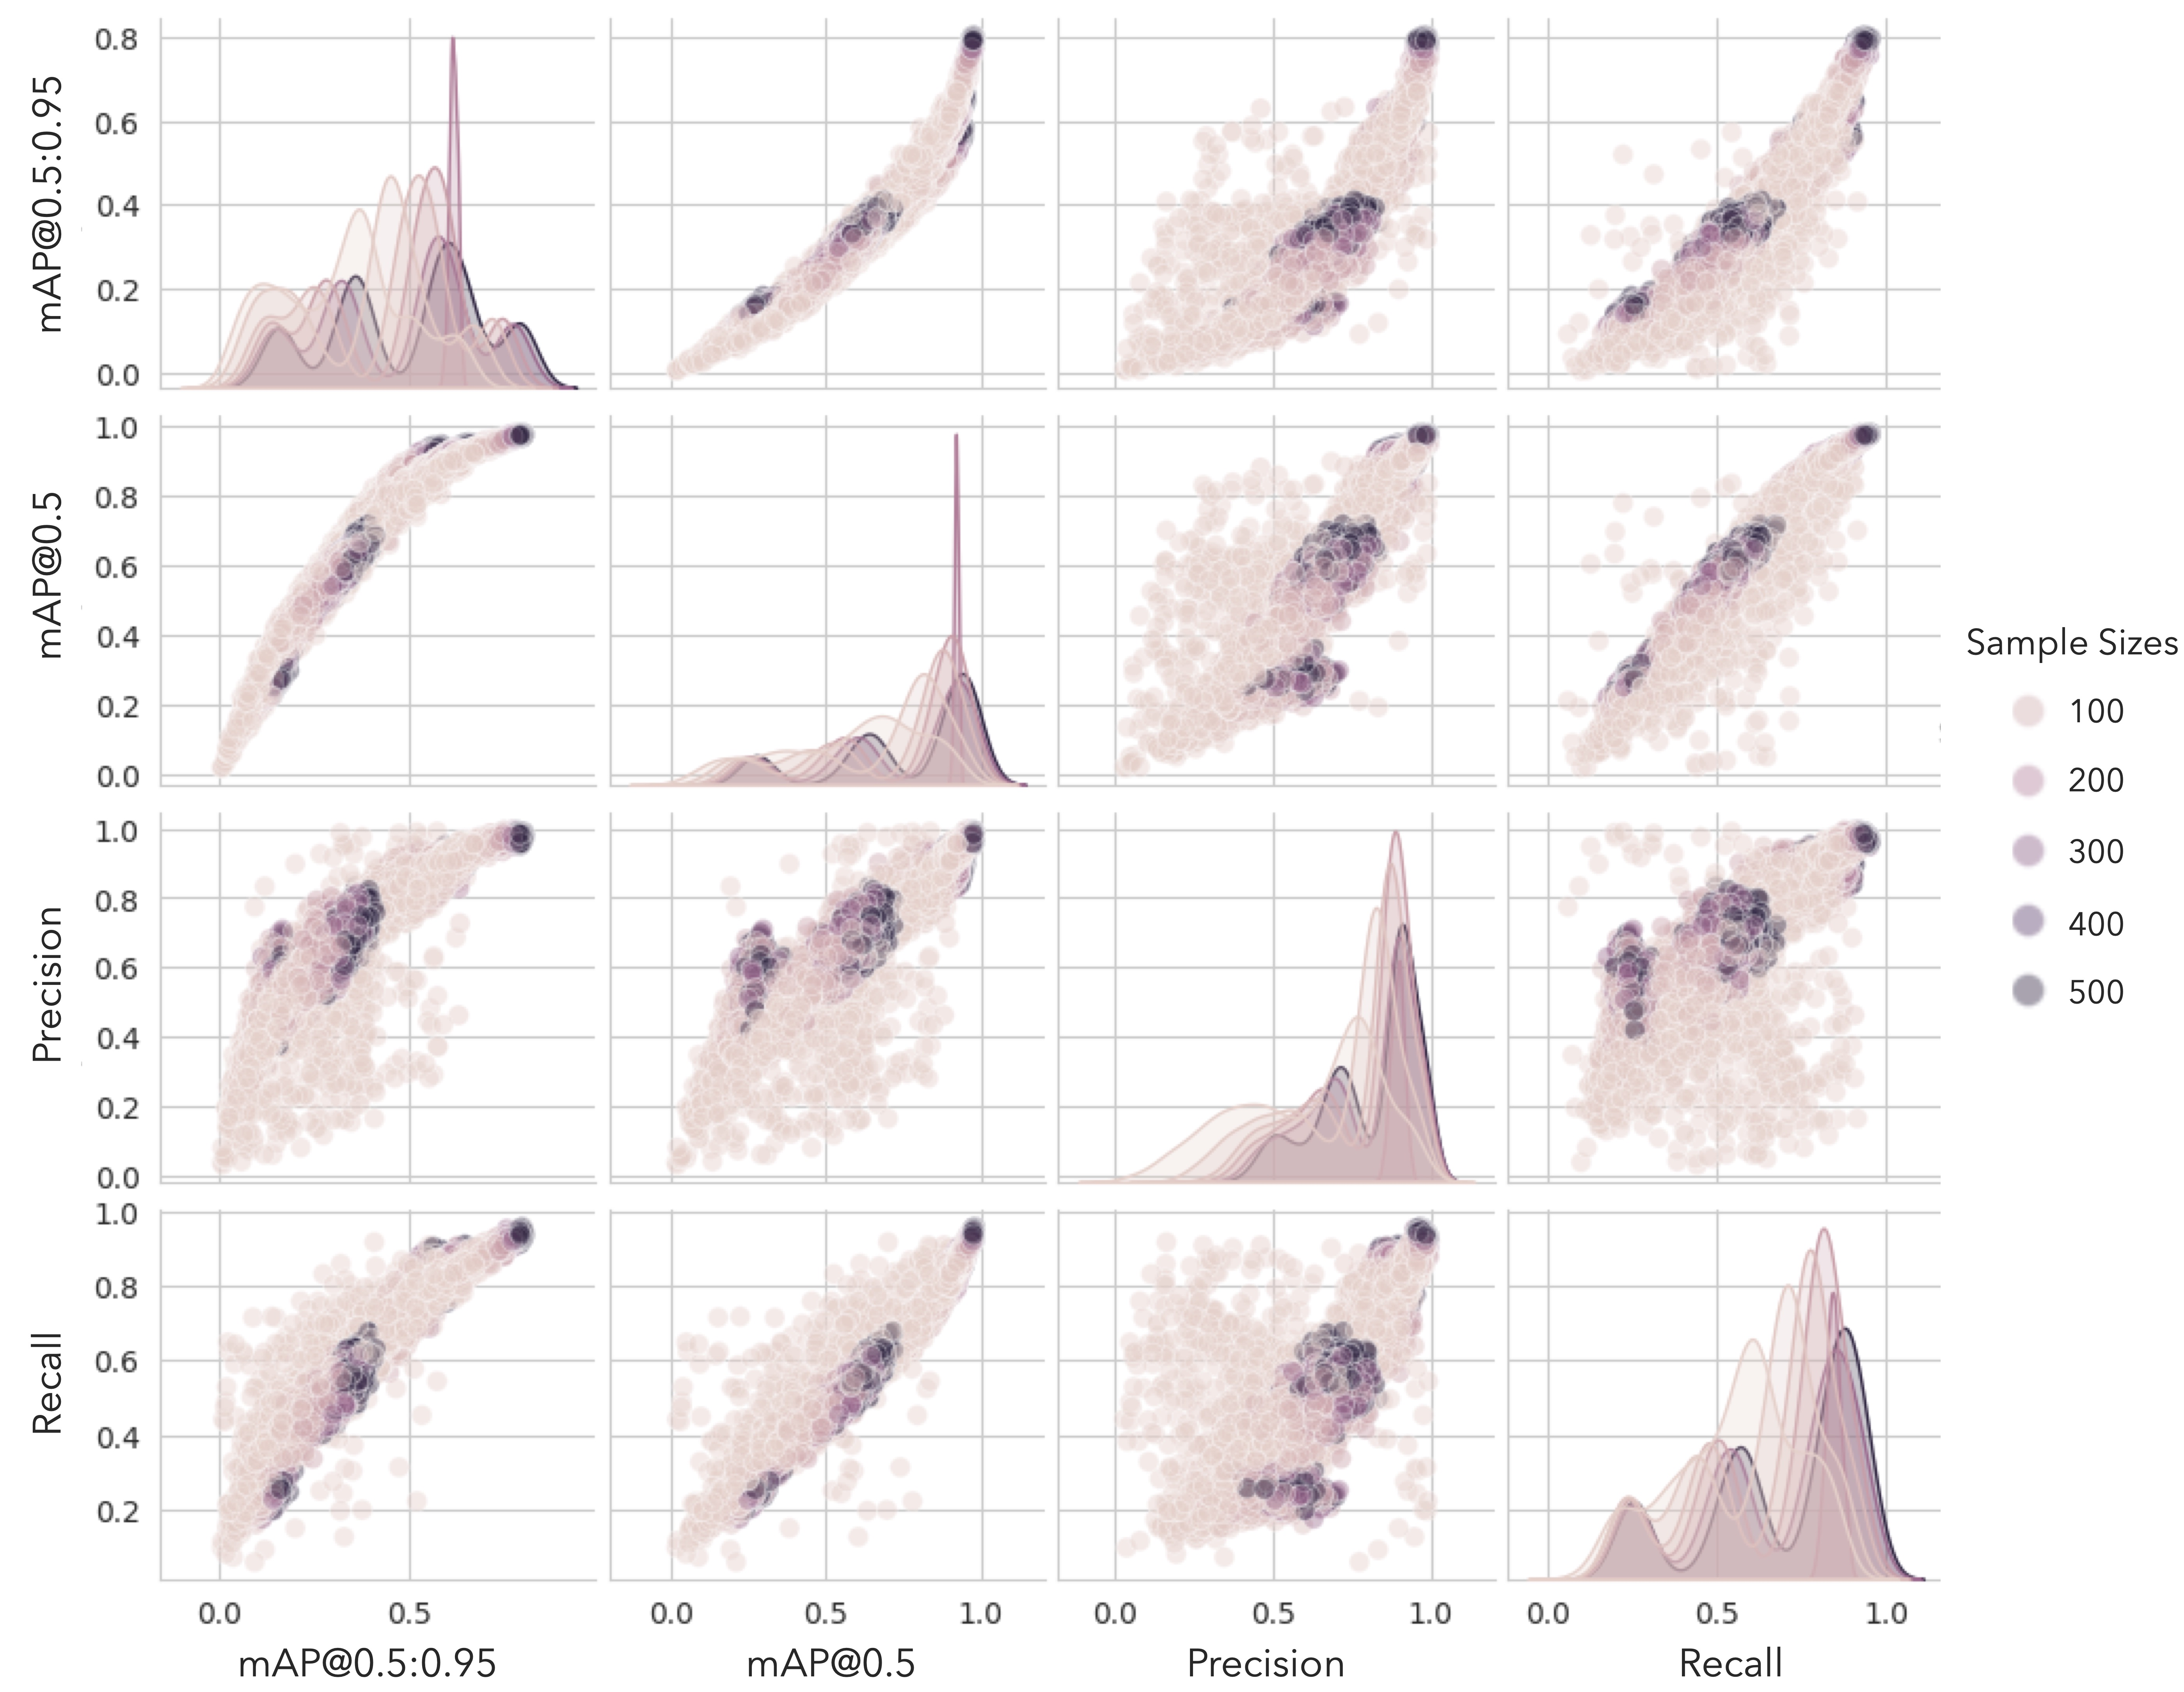
\includegraphics[width=1\textwidth]{figure_s1.jpg}
    \caption{Examples of the annotated images.}
    \label{fig:metrics}
\end{figure}



\subsection*{Study 1: The changes in camera view angles dramatically affect the model performance}


\begin{figure}[H]
    \centering
    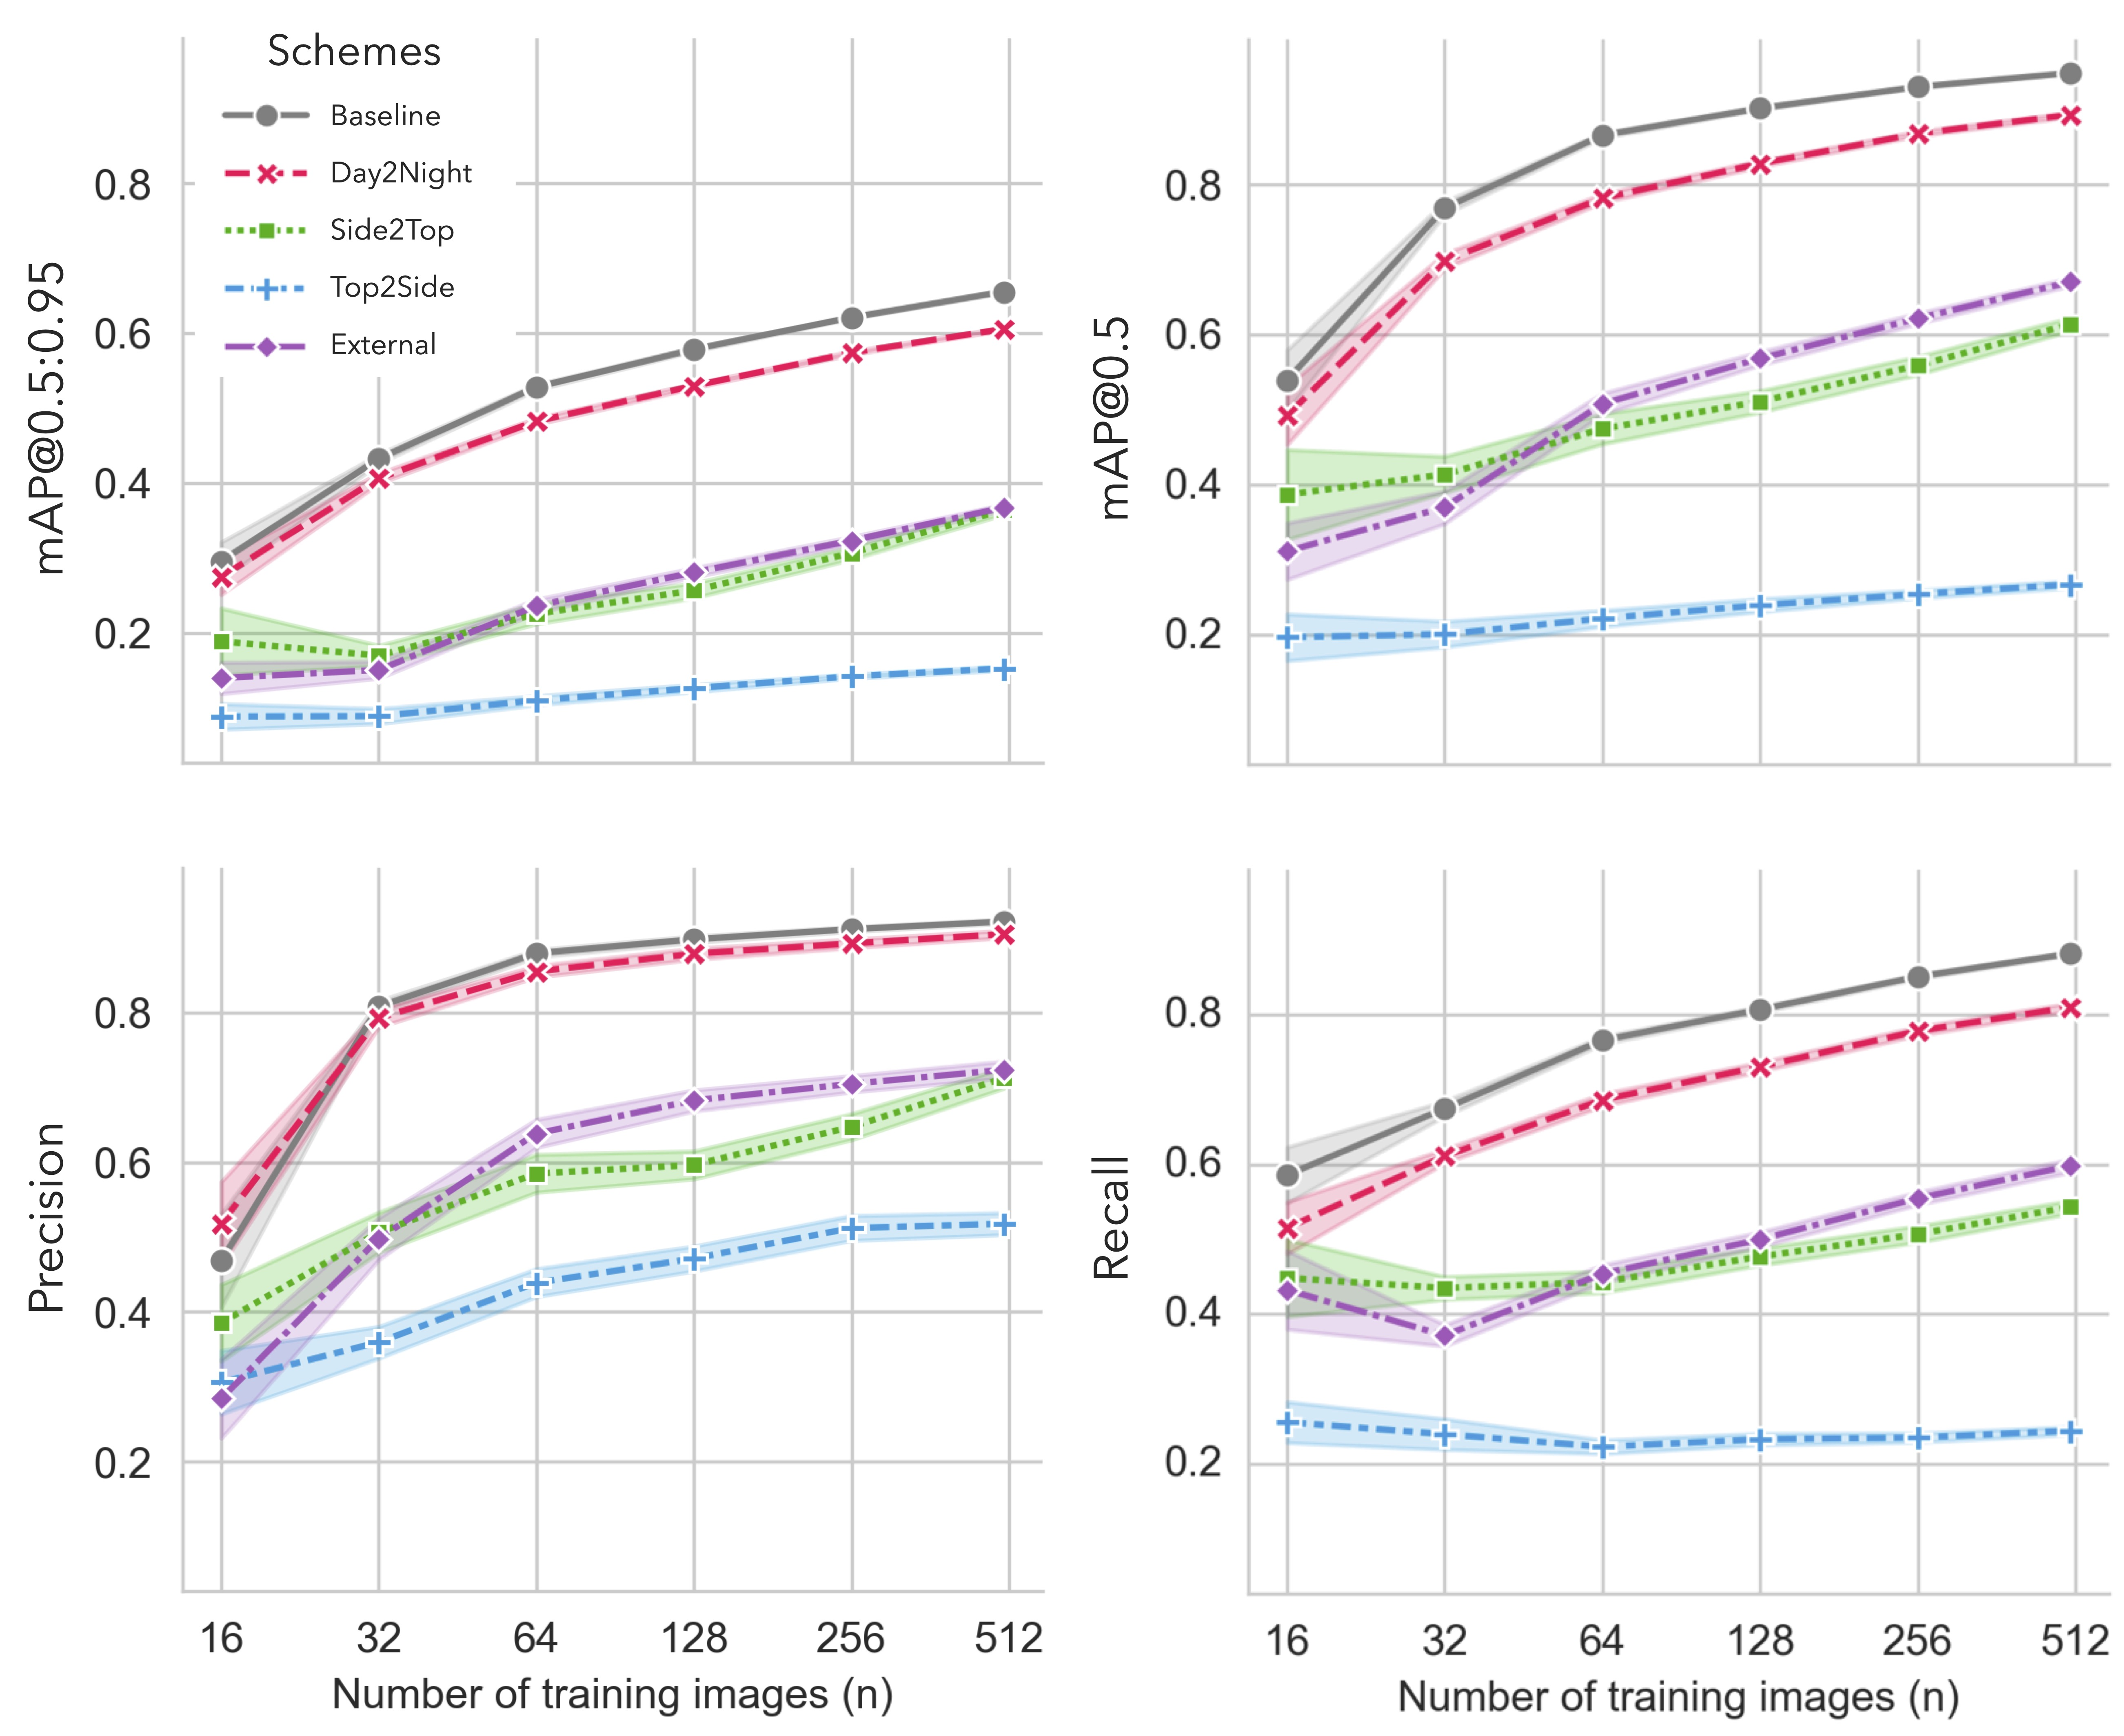
\includegraphics[width=0.8\textwidth]{figure_3.jpg}
    \caption{Examples of the annotated images.}
    \label{fig:schemes}
\end{figure}

The baseline training configuation show a good generalization capabiltiy, in which over 90\% of the predctions were correct in positioning cows at the criteria of 50\% IoU ($\text{mAP@{0.5}}$). Further, the generalization performance can be dissected into changes in view angles (i.e., Top2Side and Side2Top) and lighting condition (i.e., Day2Night). The lightinig condition changes did not dramatically affect the model performance in all four metrics, while changing camera views drop the performance by approxmiately 30\% and 60\% in ($\text{mAP@{0.5}}$ in the configurations of Side2Top and Top2Side, respectively. Across all the metrics and training sample sizes, the configuration of Top2Side consistently showed the worst performance. From the perspective of precision and recall, changing camera from top view to side view result in the model missing detecting more than 7 cows for ever 10 cows and only 50\% of the detection were correct. It is noted that the performance in the Day2Night configuration is closed to the baseline in the metric precision, which only consider predictions with high confidence compared to the metric ($\text{mAP@{0.5}}$). Hence, by excluding the low-confidence predictions, changing ligthing condition did not affect the model performance. Regardless of the configuration and the evaluation metrics, the model performances always increase as the trianing sampel sizes increase.


\subsection*{Study 2: A higher model complexity does not always lead to better performance}


\begin{figure}[H]
    \centering
    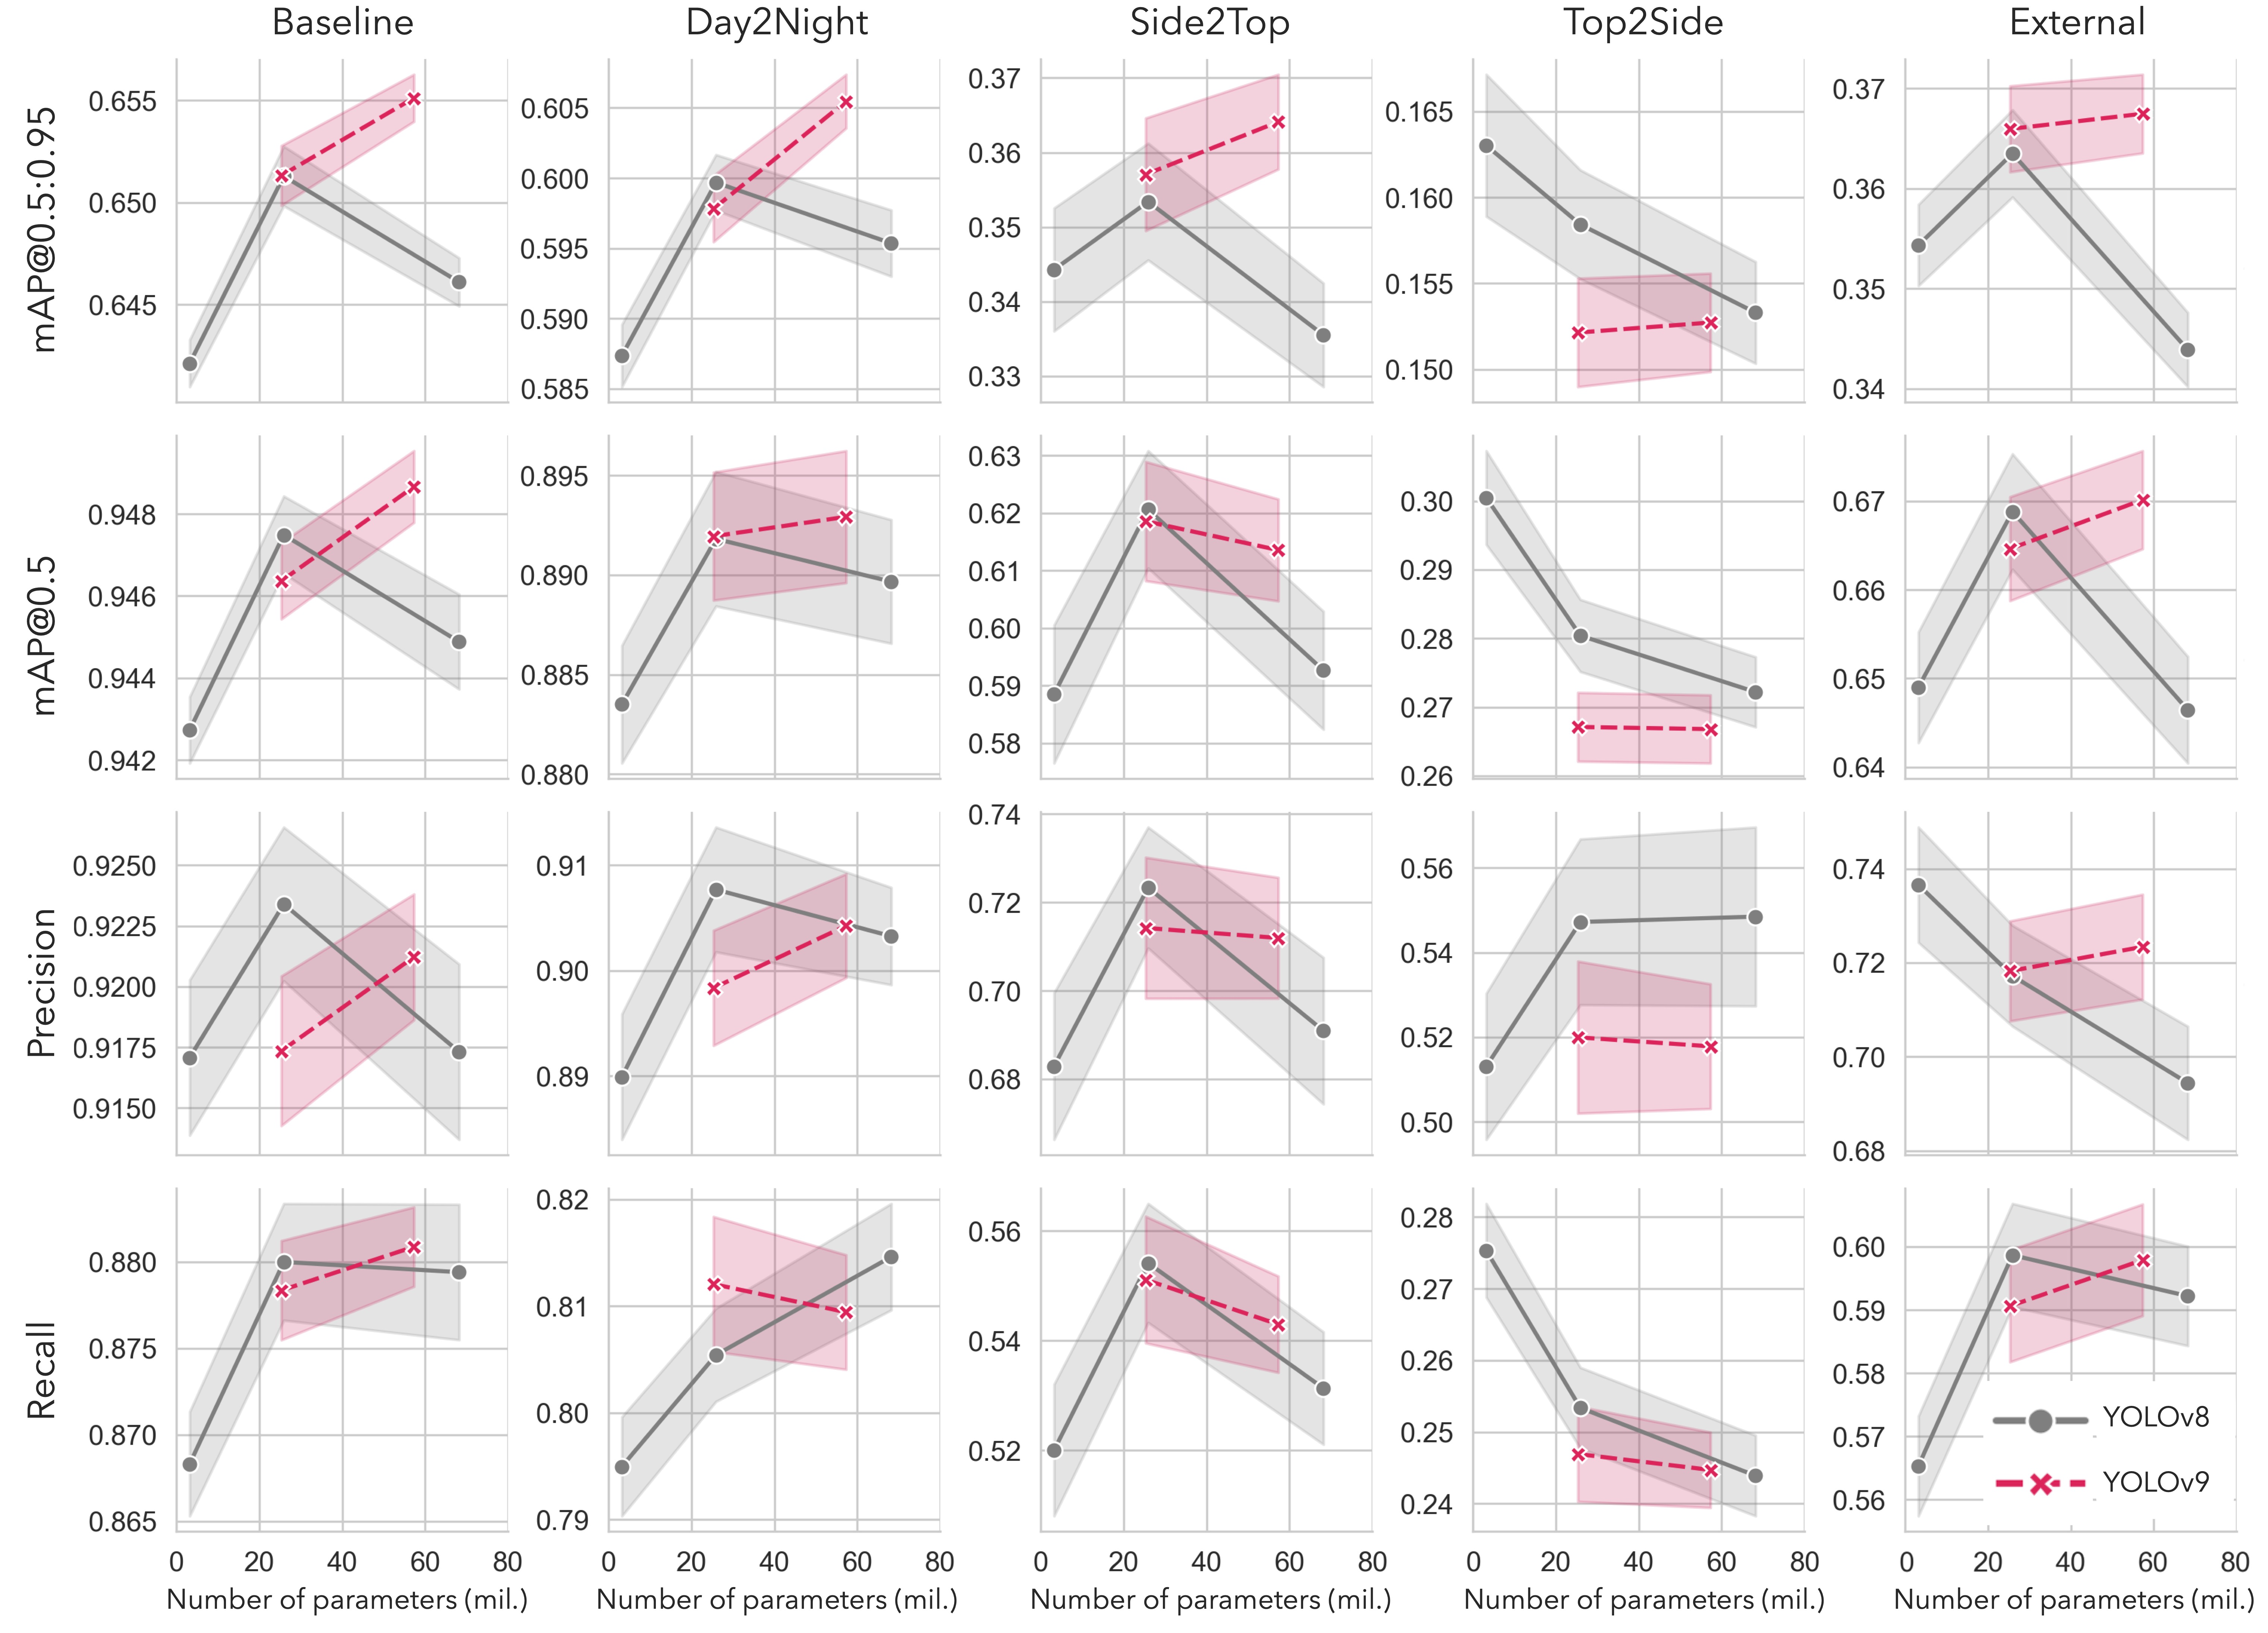
\includegraphics[width=1\textwidth]{figure_4.jpg}
    \caption{Examples of the annotated images.}
    \label{fig:models}
\end{figure}


From the study, it is found that the xxx of the training configuration affects the relationship between the model complexity and the performance. Based on the study 1, predicting images from the side view based on the model trained on from the top-view camera is the most challenging tasks. In this configuration, increasing the model complexity, except for few cases, the model generalization always became worse than the simple models are. However, in other configurations that show better generalization in the Study 1, the peak performance did not always found from the most complex model. For example, in the baseline, the model that performed that best is YOLOv9e in metrics of $\text{mAP@{0.5:0.95}}$, $\text{mAP@{0.5}}$, and recall. And YOLOv8m performed the best in precision. Neither of the model has the most parameter counts compared to YOLOv8x. It is also worth noting that, different model architecture show different trend in the performance over model complexity. The YOLOv8-family models more likely to have the best performance with the mid-sized model (i.e., YOLOv8m). While in YOLOv9, larger models usually performed better. Hence, the study concluded that the model performacne is determined by both training configuration and the model archtecture.

The required computational resources can be evaluated from training time (Figure ~\ref{fig:resources}a), inference time (Figure ~\ref{fig:resources}b), adn the memory storage sizes (Figure ~\ref{fig:resources}c). The training time was presented as a ratio of the actual training time over the baseline, which is the time required to train the YOLOv8n model with only 32 samples. The results suggested that using the largest model, YOLOv8x, that with 20 times more parameters, the training time increased by 4 to 6 times based on the training sample size. Additionally, the YOLOv9 models overall required more training time and slower inference frames per seconds (FPS) compared to the YOLOv8 models. The gap of the training time was expanded as the training samples increased. The inference time was calculated as the average FPS in a batch of 64 images. Running the models on CPU with the smallest model (i.e., YOLOv8n), was found to be slower than running the largest model (i.e., YOLOv8x) on GPU, where the FPS were 19.77 and 29.21, respectively. The importance of high FPS models was highlighted in this study, as a real-time inference usually requires a model with FPS higher than 30. Implementing these YOLO models on CPU may not meet this goal according to the result.


\begin{figure}[H]
    \centering
    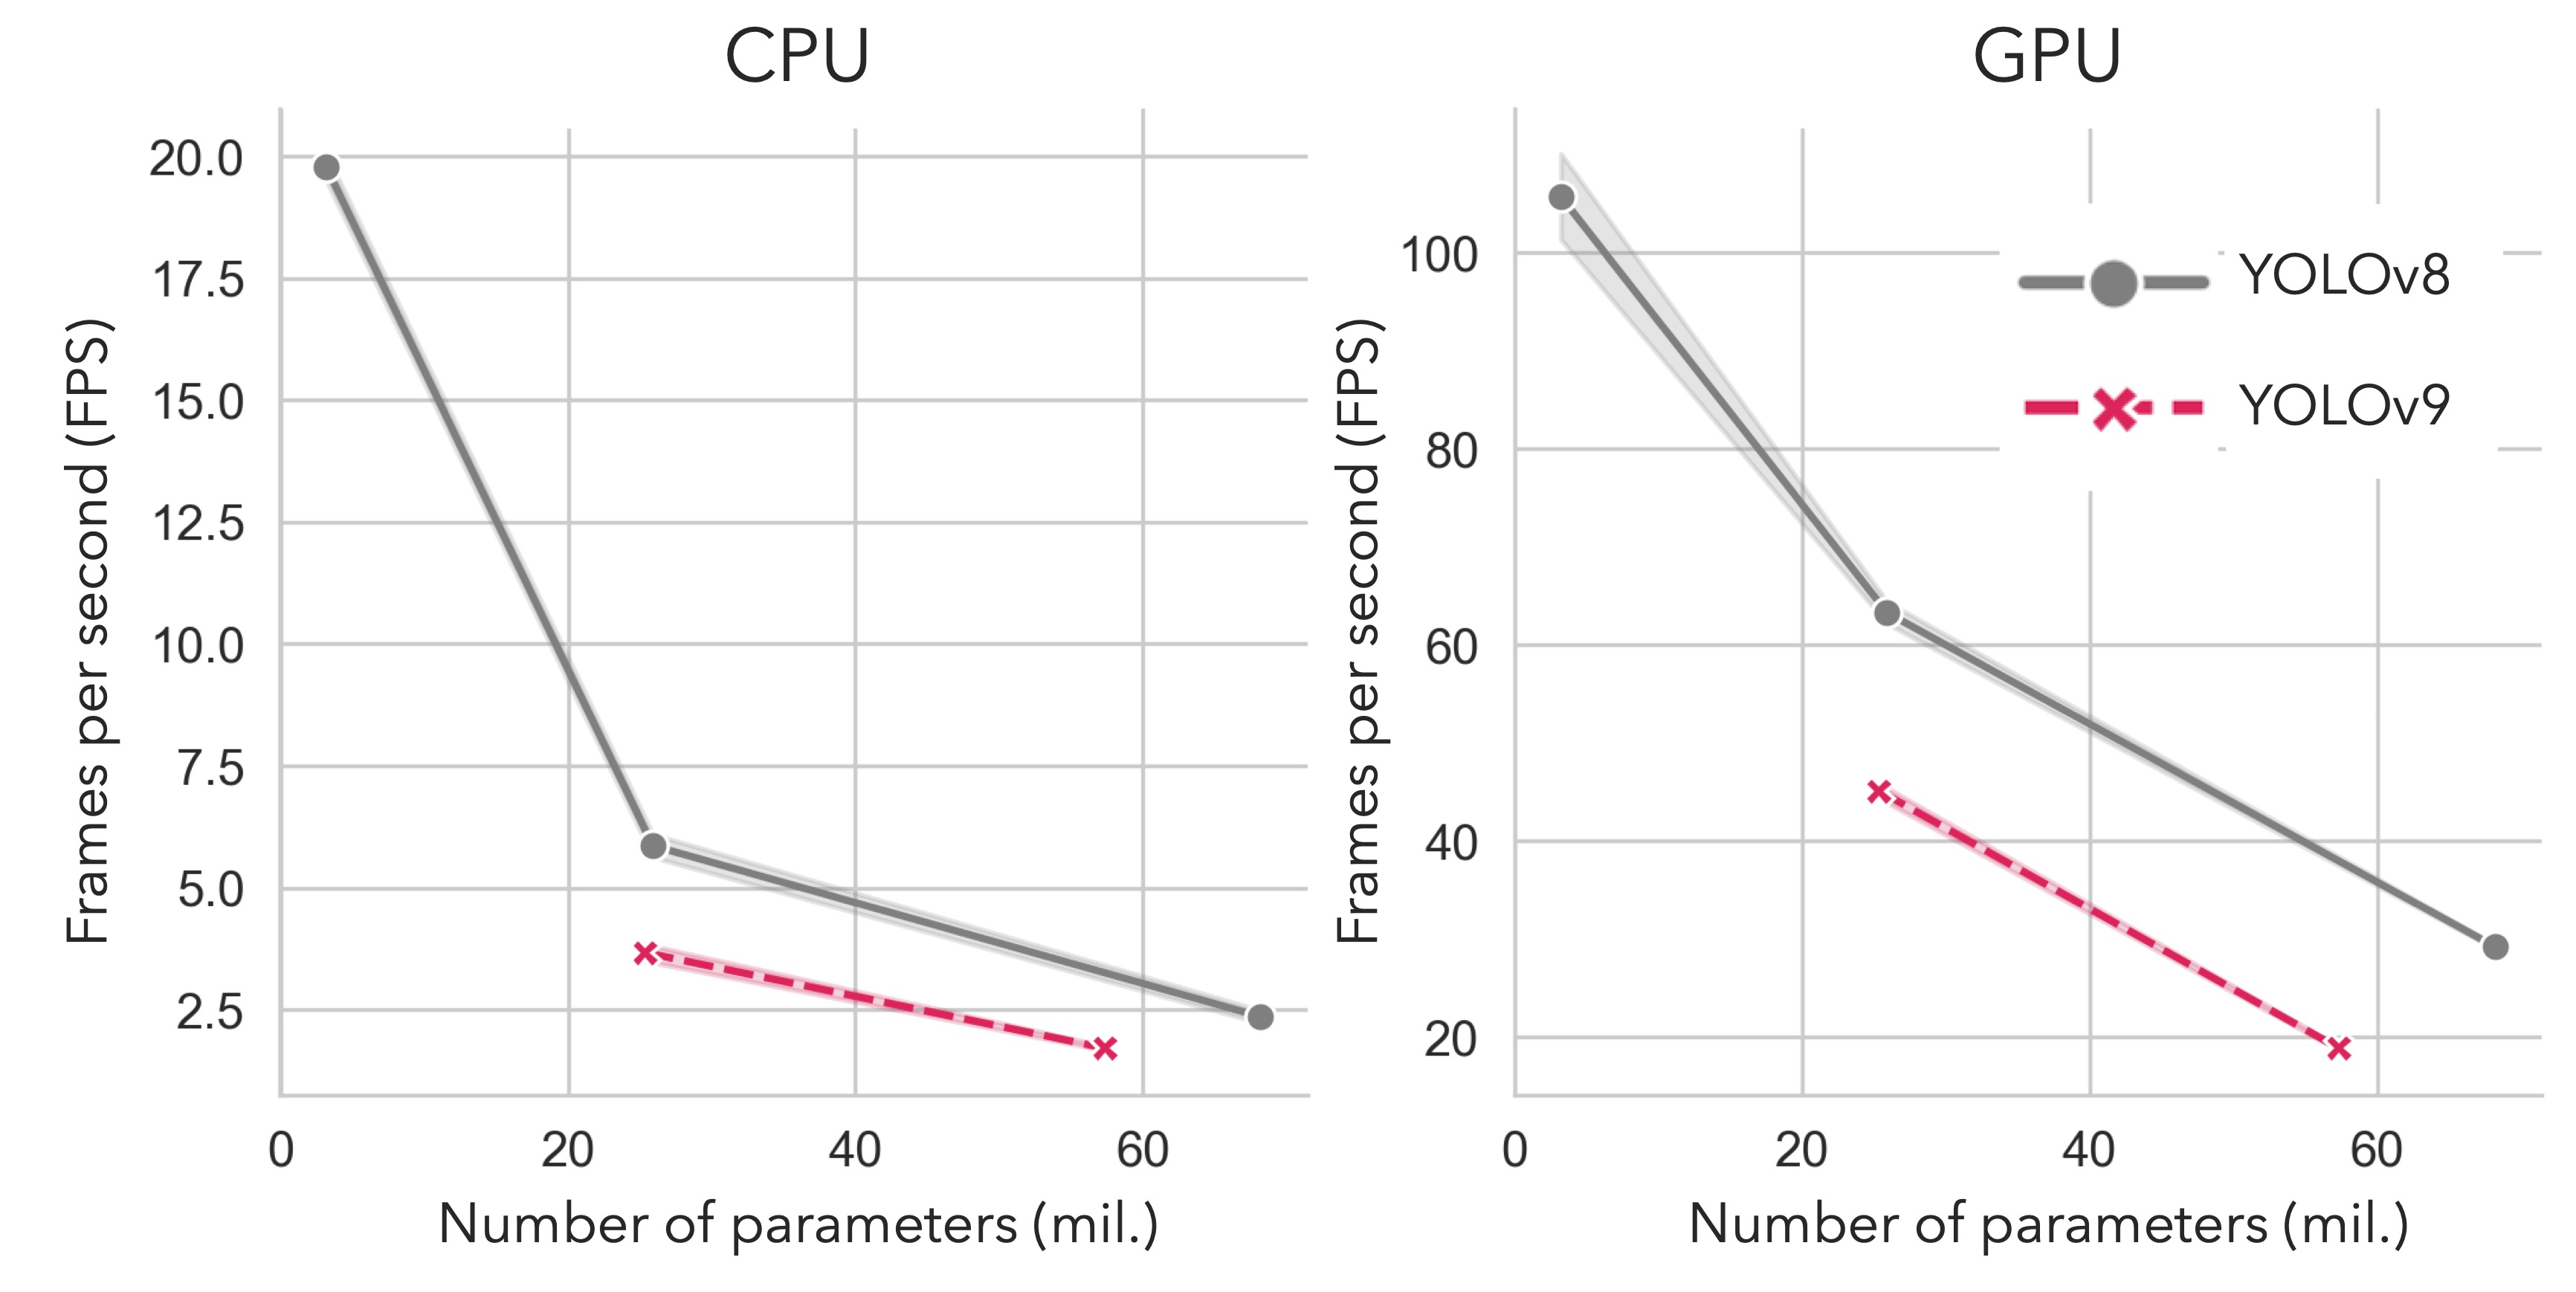
\includegraphics[width=1\textwidth]{figure_6.jpg}
    \caption{Examples of the annotated images.}
    \label{fig:resources}
\end{figure}


\subsection*{Study 3: The advantages of fine-tuning the model is limited when the model is simple}

The results presented in Figure \ref{fig:finetune} indicate that the benefit of using fine-tuned initial weights is minimal for simpler models. Specifically, when employing YOLOv8n, the performance difference between the default and fine-tuned weights was insignificant when fine-tuning data from the Top-View Camera and Side-View Camera. However, as the model complexity increased, a greater number of fine-tuning samples were required for the two different initial weights to achieve similar performance. For instance, in the case of YOLOv9e, the performance gap was eliminated when the number of fine-tuning samples reached 128 and 64 for the Top-View Camera and Side-View Camera data sources, respectively. The similar trend was observed from the External camera, where a significant performance gap of more than 25\% in mAP50:95 was observed for YOLOv9e when the sample size was 16. It is also noted that, although the performance gap was closed to zero from the Top-View Camera and Side-View Camera data sources, the gap was never closed for the External camera. In summary, using fine-tuned initial weights is only beneficial for models with larger parameter sizes (e.g., YOLOv8x, YOLOv9c, and YOLOv9e) and when limited training samples are available.

\begin{figure}[H]
    \centering
    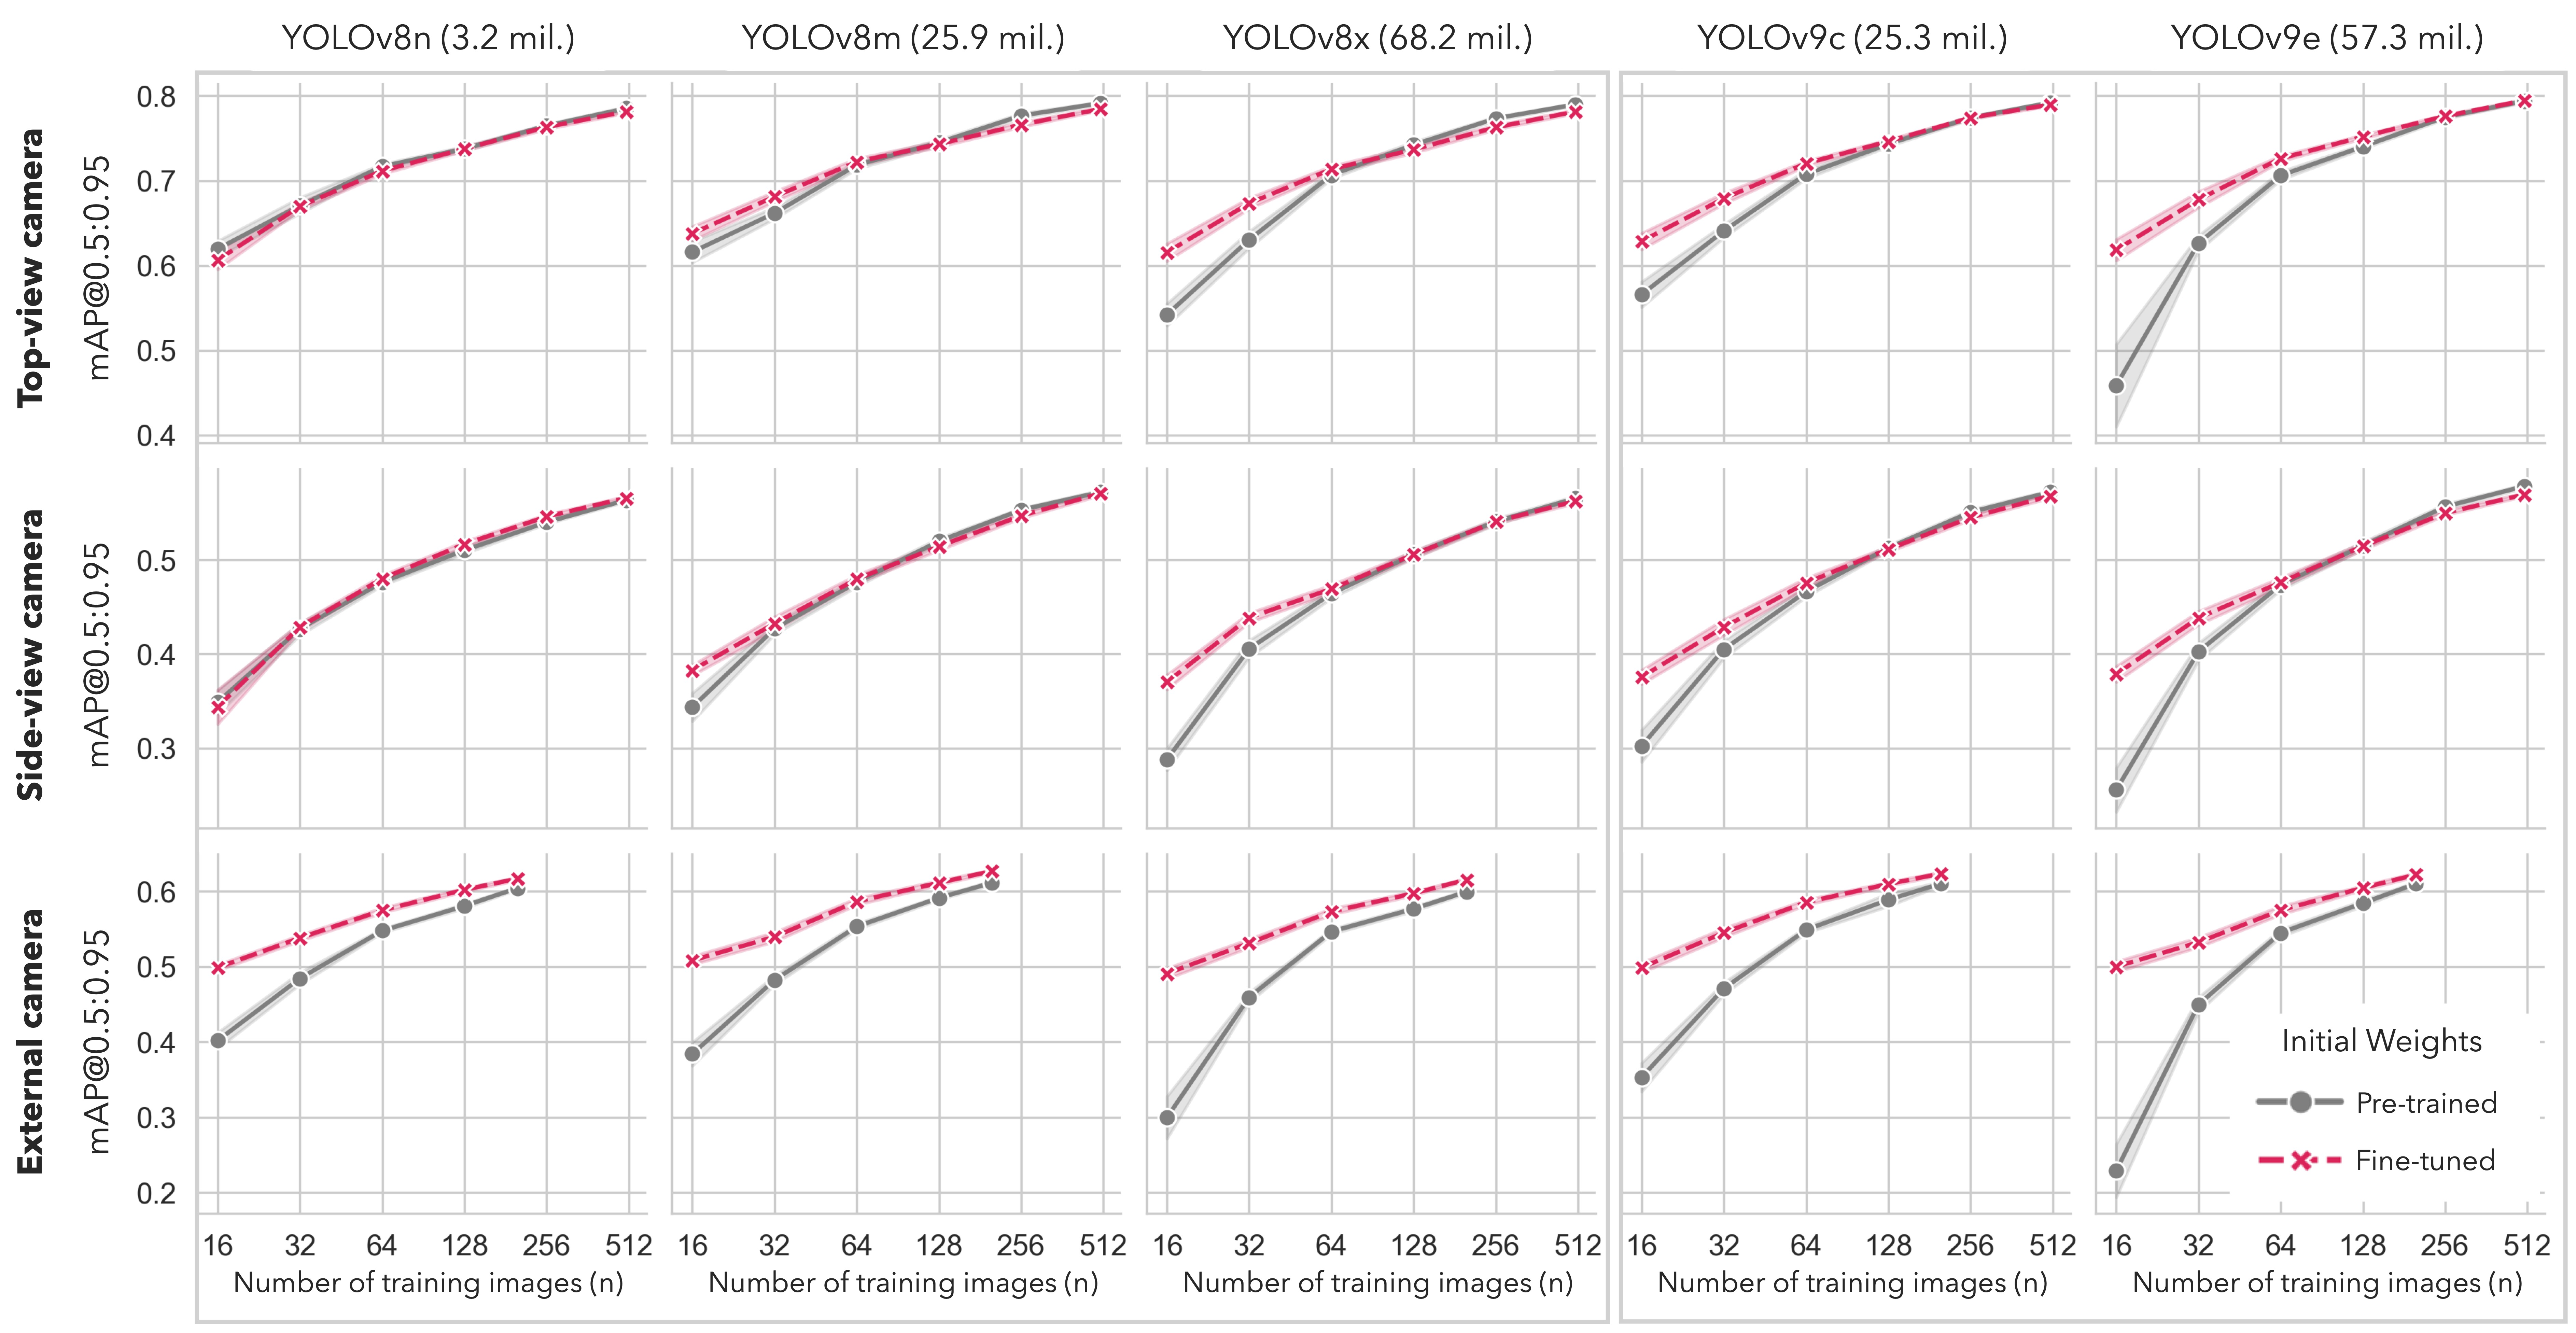
\includegraphics[width=1\textwidth]{figure_5.jpg}
    \caption{Examples of the annotated images.}
    \label{fig:finetune}
\end{figure}

